
\chapter{Aglomerado de Galáxias}
A origem do Universo, de acordo ao modelo cosmológico padrão, se deu há aproximadamente 14 milhões de anos. Desde então o seu processo de expansão ocorre de forma contínua e hierárquica, de modo que unidades menores se fundem formando outras maiores. Aglomerados de galáxias são as maiores estruturas do Universo observável e compõem os objetos de estudo desta dissertação.  

Aglomerados de galáxias são definidos basicamente por três componentes: galáxias, meio intra-aglomerado e matéria escura. A maior parte da massa do aglomerado, cerca de 80\% do total, é composta de matéria escura (não-bariônica). Do restante, na forma bariônica (feita de prótons e nêutrons), 15\% são compreendidos de gás intra-aglomerado (MIA) e apenas 5\% da massa de um aglomerado estão na forma de estrelas de galáxias.

A busca por compreender a formação e evolução dos aglomerados de galáxias é uma das questões mais importantes da Astrofísica. No paradigma atual de formação das estruturas, as galáxias e os aglomerados surgem a partir de halos escuros. O resfriamento desses halos ocasiona a formação de estruturas condensadas, onde depois colapsariam os bárions, formando  os sistemas astrofísicos conhecidos. Este cenário seria ainda hierárquico, com a formação dos aglomerados ocorrendo após a formação das galáxias, aproximadamente em um desvio para o vermelho $z \approx 2$ (Velásquez, 2007).

\begin{figure}[!htb]
	\centering
	\caption{Histograma de velocidades no Aglomerado.}
	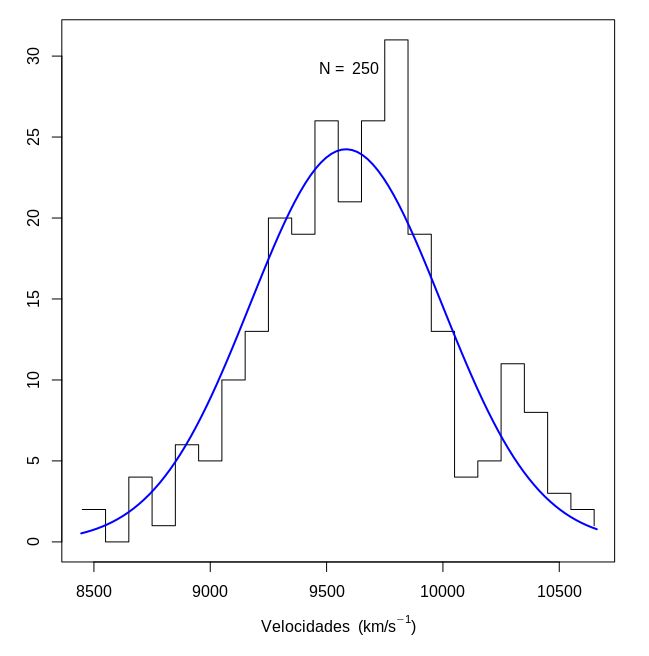
\includegraphics[width=0.3\textwidth]{04-figuras/distVel}
	\fonte{Autor}
	\label{fig1}
\end{figure}

O processo de formação de aglomerados de galáxias ainda não atingiu o seu fim. Enquanto regiões centrais estão em equilíbrio dinâmico, as regiões periféricas (externas) acumulam matéria na forma de galáxias ou grupos de galáxias de modo contínuo. Comumente o entorno dos aglomerados de galáxias é constituído de grupos de galáxias que podem ser absorvidos pelo aglomerado principal ao longo do tempo, ocasionando o aumento de sua massa (Rembold, 2011). Estudos sobre a distribuição de velocidades de galáxias em aglomerados indicam que a mesma possui distribuição Não Rejeita, vide Figura \ref{fig1}, ou muito bem ajustada por uma gaussiana somente na região virializada do sistema (região mais interna do sistema) (Yahil \& Vidal 1977), podendo existir sinais de múltiplos modos normais na região mais externa (Ribeiro, Lopes \& Trevisan 2011), comprovando a presença de componentes de um sistema em processo de evolução pelo acréscimo de matéria ao seu entorno. Esse acréscimo de matéria, na forma de galáxias ou grupo de galáxias.  Isto sugere que a formação de aglomerados de galáxias é um processo contínuo que decorre de fusões sucessivas e encontros gravitacionais de maiores e menores proporções (Nascimento et al., 2016).



\section{Distribuição de Velocidades ao longo do Aglomerado}
A velocidade de uma galáxia contida em um aglomerado, em uma dada posição, não pode ser maior que a velocidade de escape do sistema, caso isto aconteça a galáxia não pertenceria mais ao aglomerado. A velocidade de escape e a distância ao centro do aglomerado são grandezas inversamente proporcionais, ou seja, a velocidade de escape decresce com o aumento da distância ao centro do aglomerado, portanto é mais fácil o escape de uma galáxia que está na região periférica (de Oliveira e Viegas, 2004).

Para que o aglomerado exista como unidade dinâmica é preciso uma redução na amplitude da distribuição de velocidades das galáxias à medida que haja um afastamento da região central. O grande problema dessa propriedade é o efeito de projeção. As galáxias que estão com distâncias distintas do centro do aglomerado podem parecer ao observador com mesma distância em consequência da observação apenas das posições projetadas no plano do céu (de Oliveira e Viegas, 2004).

Na Figura \ref{fig2} vemos a distribuição de velocidades do aglomerado em função da distância da galáxia ao centro do aglomerado, onde o estreitamento da distribuição de velocidades define uma espécie de "corneta" que pode ser utilizada para definir os membros de um aglomerado, sendo removidas as galáxias que estejam significativamente acima ou abaixo da "corneta".

\begin{figure}[!htb]
	\centering
	\caption{Distribuição de velocidades em função da distância ao centro do Aglomerado.}
	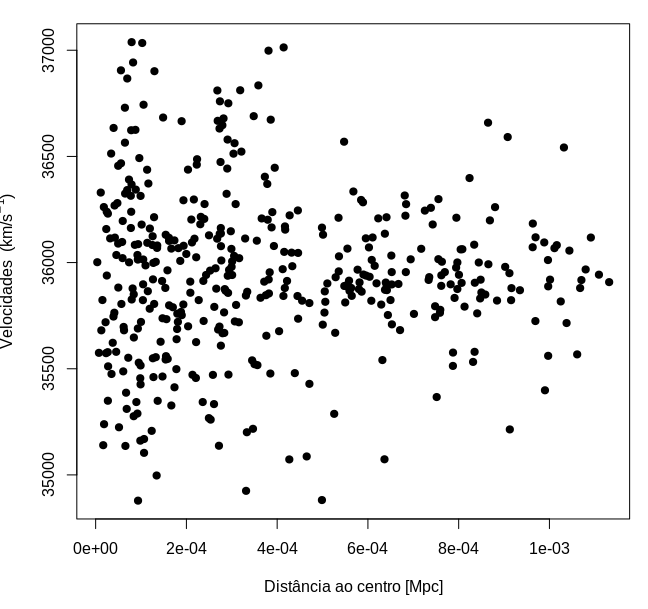
\includegraphics[width=0.3\textwidth]{04-figuras/distCenter}
	\fonte{Autor}
	\label{fig2}
\end{figure}

\chapter{Rotação de Aglomerados}

O conhecimento do estado dinâmico de aglomerados de galáxias pode propiciar restrições importantes em cenários cosmológicos, como a determinação da massa total do aglomerado e uma estimativa da quantidade de matéria escura no Universo. A possibilidade da existência de aglomerados em rotação tem sido discutida por muitos autores (por exemplo, veja os estudos de Hwang \& Lee 2007; Manaloupoulos \& Plionis 2016). 

Para detecção de indícios de rotação, Hwang \& Lee (2007) utilizaram dados espectroscópicos do \textit{Sloan Digital Sky Survey} \footnote{Considerado o mais ambicioso mapeamento astronômico que já foi feito. Com este mapeamento, os astrônomos podem observar os padrões de grande escala das galáxias: filamentos e vazios em grandes regiões angulares do Universo.}(SDSS) e \textit{Two-Degree-Field Galaxy Redshift Survey} (2dF-GRS). A rotação de aglomerados foi modelada como a rotação de galáxias membro e a rotação do gás intra-aglomerado. Eles levantaram inicialmente a hipótese de que a rotação se origina através de fusões de aglomerados. Um aspecto importante do método empregado por Hwang \& Lee (2007) é que os aglomerados com rotação devem exibir divisão espacial entre galáxias com velocidades maiores e menores que a velocidade média do aglomerado além de apresentar um pico no mapa de densidade. Nesta pesquisa de Hwang \& Lee (2007) foram detectados seis sistemas com rotação, em um total de dozes aglomerados (Abell 0954, Abell 1139, Abell 1399, Abell 2162, Abell 2169, and Abell 2366). Constatou-se ainda que estes aglomerados estão em equilíbrio dinâmico e não sofreram fusão recente, não dando suporte, portanto, à hipótese de interações como causadoras da rotação. 

Kalinkov et al. (2008) tentaram obter o gradiente máximo no campo de velocidades de Abell 2107 e determinaram que a direção do coeficiente de correlação linear máximo definiria o eixo maior do aglomerado e o eixo menor seria o de rotação. Foram utilizadas subamostras de galáxias membro, ordenadas de acordo a distância ao centro do aglomerado para definir o grau de rotação do sistema. Esse mesmo aglomerado foi estudado por Oegerle et al. (1992) e foram encontrados indícios de rotação. Materne et al. (1983) apontaram a dificuldade em diferenciar um aglomerado rotativo de dois que se sobrepõem, pelo motivo de estar se fundindo ou se afastando. Porém, o aglomerado  Abell 2107 não consiste de dois aglomerados sobrepostos, em consequência do pico estreito representado em seu histograma de velocidades. O indicador mais forte que definiu a rotação foi o ângulo de posição do eixo com o gradiente máximo no campo de velocidades quase coincidindo com o ângulo de posição do eixo com o maior alongamento.  Nesse estudo o período de rotação foi calculado em uma volta a cada $2.4\times10^9$ anos e houve uma correção no valor da massa para $2.8\times10^{14}~{M_\odot}$  (a massa inicial era de $3.2\times10^{14}~{M_\odot}$, sem levar em conta a rotação). 

Baseado no estudo da distribuição de velocidades das galáxias membro, Tovmassian (2015)  detectou sinais de rotação em 17 de uma amostra de 65 aglomerados (26\%). O método analisa o número de galáxias com velocidades mais baixas e mais altas que a velocidade média do aglomerado em diferentes partes do aglomerado. O método teve mais êxito em aglomerados planos, com $f=a/b > 1.8$ (a e b semieixos - maior e menor – da distribuição de galáxias do aglomerado). 
Para estes, a taxa de detecção de rotação foi mais alta (7 dos 18 aglomerados planos, 39\%).  Esse resultado suporta a opinião de que os aglomerados foram originalmente formados a partir das enormes nuvens de gás primordiais e preservaram a rotação das nuvens primordiais, a menos que sofram fusões com outros aglomerados e grupos de galáxias. 

Já na tese de Manolopoulou (2014) é realizado um estudo de um novo algoritmo para dedução de rotação usando a velocidade radial projetada\footnote{É a velocidade de um objeto na direção da linha de visada, isto é, a velocidade com que o objeto se aproxima ou se afasta do observador.}. Inicialmente os testes foram realizados em aglomerados gerados em simulações de Monte Carlo para confirmar se o método fornecia indicações robustas de rotação. Em seguida, aplicado em amostras de aglomerados de Abell. Através do teste de Kolmogorov-Smirnov, decidiu-se quanto a sua rotação significativa ou não, seu centro rotacional, orientação do eixo de rotação, amplitude de velocidade rotacional e, finalmente, o sentido de rotação no sentido horário ou anti-horário no plano do céu. Foram encontrados 23 aglomerados possivelmente rotativos dentro de 1.5 Mpc ou a uma distância de 2.5 Mpc do centro do aglomerado, do total de 45 da amostra.

\chapter{Ferramentas Estatísticas Utilizadas}
\section{Teste de Hipótese}
A análise estatística objetiva, especialmente, fazer inferência sobre uma população a partir da observação de uma amostra. Os testes de hipótese representam uma forma de inferência estatística. A hipótese é uma afirmação sobre parâmetros populacionais que devem ser analisadas para verificar sua veracidade. É importante ressaltar que a verdade ou não nunca pode ser determinada, a menos que toda a população seja observada, situação impraticável na maioria das vezes, justificado pelo uso do teste estatístico.  

A princípio é necessário estabelecer como verdadeira a \textbf{hipótese nula}, denotada por \textbf{$H_0$}. Já a \textbf{hipótese alternativa ($H_1$)}, contrapõe a hipótese nula, ou seja, $H_0$ deverá ser rejeitada. É necessário estabelecer um critério auxiliar para decidir a rejeição ou não de $H_0$ para um teste estatístico. Esse valor, determinado pelo pesquisador antes da análise de dados ou até mesmo na coleta de dados, cenário ideal, é denominado \textbf{nível alfa ($\alpha$) ou nível de significância}. Comumente é utilizado como critério de rejeição uma probabilidade de 5\%. De acordo com Cramer e Howitt (2004), 

\begin{citacao}
O nível em que a hipótese nula é rejeitada é geralmente definido como 5 ou menos vezes fora de 100. Isso significa que tal diferença ou relacionamento é provável que ocorra por acaso 5 ou menos vezes de 100. Este nível é geralmente descrito como proporção 0.05 e às vezes como a porcentagem 5\%. O nível de probabilidade de 0.05 foi historicamente uma escolha arbitrária, mas tem sido aceitável como uma escolha razoável na maioria das circunstâncias. Se houver um motivo para variar este nível, é aceitável fazer então. Então, em circunstâncias em que pode haver consequências adversas muito graves se a decisão errada foi feita sobre a hipótese, então o nível de significância poderia ser mais rigoroso em, digamos, 1\% (Cramer and Howitt, 2004: 151). 
\end{citacao}

Na realização de testes de hipóteses é possível que erros sejam cometidos, como mostrado no quadro \ref{qua:hipotese}. \textbf{Erro do tipo I}, denotado por \textbf{erro $\alpha$}, a rejeição de $H_0$ quando ela é verdadeira. Contrapondo, a não-rejeição de $H_0$ quando esta é falsa é denominada \textbf{erro do tipo II} e representado por \textbf{$\beta$}.  Esse tipo de teste permite concluir se deve aceitar ou rejeitar a hipótese nula, porém não é possível quantificar o quão provável é o resultado de ocorrer ao acaso. Apoiado por isto, é definido a potência de um teste estatístico $1-\beta$ como a probabilidade de rejeitar $H_0$ quando de fato é falsa. Claramente, o teste ideal é aquele em que os valores de $\alpha$ e $\beta$ são mínimos. Porém, o valor de $\alpha$ é inversamente relacionado com o valor de $\beta$, sendo impossível minimizá-los simultaneamente. Geralmente, é fixado o nível de significância $\alpha$ e escolhido a região de rejeição que minimiza $\beta$, ou seja, que maximize a potência do teste. 


\begin{quadro}[!htb]
	\centering
	\caption{Tipos de erros em testes de hipótese.\label{qua:hipotese}}
	\begin{tabular}{|l|l|l|ll}
		\cline{1-3}
\multicolumn{1}{|c|}{\multirow{2}{*}{\textbf{Decisão Estatística}}} & \multicolumn{2}{l|}{\textbf{Natureza (estado verdadeiro ou desconhecido)}} &  &  \\ \cline{2-3}
\multicolumn{1}{|c|}{} & \multicolumn{1}{c|}{\textbf{$H_0$ verdadeira}} & \multicolumn{1}{c|}{\textbf{$H_1$ falsa}} &  &  \\ \cline{1-3}
\textbf{Aceitar $H_0$} & acerto & Erro tipo II ( \ensuremath{\beta}) &  &  \\ \cline{1-3}
\textbf{Rejeitar $H_0$} & Erro tipo I ( \ensuremath{alpha}) & acerto &  &  \\ \cline{1-3}
	\end{tabular}
	\fonte{\citeonline{}}
\end{quadro}

O menor nível de significância pode ser definido utilizando o \textbf{valor-p} ou \textbf{\textit{“p-value”}}. No teste de hipótese esse valor é comparado ao nível de significância \ensuremath{alpha} determinado no início objetivando a tomada de decisão de aceitar ou rejeitar $H_0$. Se o valor-p calculado do teste for igual ou maior que \ensuremath{alpha}, a $H_0$ é aceita. Ou seja, a hipótese nula é consistente com os resultados da amostra. Porém, se o valor-p for menor que \ensuremath{alpha}, a hipótese nula é rejeitada, a hipótese alternativa, nesse caso, é então aceita como verdadeira.

\section{Teste de Normalidade}
Uma variável aleatória, seja idade de um grupo de pessoas ou ocorrência de um determinado desfecho, pode admitir uma distribuição de frequências da população, contendo diversas formas encontradas na literatura estatística. O intuito desses modelos é caracterizar o comportamento de um determinado evento em função da frequência de sua ocorrência. Se as variáveis forem contínuas, o evento será um intervalo de valores. Portanto, as distribuições de frequências são efetivamente distribuições de probabilidade, em que para um evento teremos associado uma probabilidade de ocorrência (T2). 

A inspeção visual pode ser utilizada para avaliação da normalidade. A distribuição de frequência, como exemplo um histograma, relaciona valores observados à sua frequência e pode além de pressupor uma distribuição normal, identifica \textit{insights} sobre lacunas nos dados e outliers. O histograma é composto por barras justapostas em que no eixo horizontal contém a variável de interesse dividida em classes e no eixo vertical a sua correspondente frequência (T2). Para distribuições do tipo normal ou Gaussiana, o histograma constitui formato de sino (Figura 3b).

Entretanto, a simples constatação por meio de gráficos é subjetiva e não satisfatória, pois depende de uma interpretação visual além de não ser confiável no caso multivariado e especificamente nas situações de muitas variáveis. Desta forma, para inferir sobre a normalidade é necessário utilizar como complemento testes estatísticos (T1).  Como exemplo, podemos citar: o teste de aderência qui-quadrado; Kolmogorov-Smirnov; Lilliefors e Shapiro-Wilk. 

Estes testes possuem estatísticas de teste e critérios de decisão diferentes, porém compartilham da hipótese avaliada: a hipótese de nulidade ($H_0$) especifica que a variável aleatória adere à distribuição normal, sem a necessidade de definir a média ou variância da distribuição. Já a hipótese alternativa ($H_1$), opõe a hipótese nula (T2). 

O resultado que interessa após executar um determinado teste é o seu valor-p ou nível descritivo do teste, referente à probabilidade de que a estatística do teste (como variável aleatória) tenha valor extremo em comparação ao valor observado (estatística) quando a hipótese nula é verdadeira. Sendo o valor-p menor que o nível de significância, logo a hipótese nula é rejeitada. Ou seja, o valor-p representa o menor nível de significância que pode assumir para então rejeitar a hipótese nula. Logo, há significância estatística quando o valor-p é menor que o nível de significância estabelecido (FLÁVIO – ESTUDO DA DISTRIBUIÇÃO).  

\section{Testes utilizados}
\subsection{Teste de Cramer-von Mises}
Em estatística, o teste de Cramér (conhecido também como phi de Cramer - $\varphi$c) é uma medida de associação entre duas variáveis nominais dado o intervalo de 0 a 1, indicando que um valor mais alto possui forte associação. Fundamentado no teste estatístico do qui-quadrado de Pearson, foi publicado em 1946 por Harald Cramér. A medida é definida como

\begin{equation}
\ V = \sqrt{\frac{{\chi_{obt}}^2}{N.m}}
\label{eq:eq1}
\end{equation}
	
	onde $\chi^2$ é o valor obtido do teste estatístico
	
	N é o tamanho da amostra e 
    
    m = o menor de (r - 1) ou (c – 1), sendo r o número de linhas e c o número de colunas.

Para entender melhor a utilidade do teste de Cramer é fundamental compreender as formas como os testes estatísticos divergem das medidas de associação para variáveis categóricas. O teste qui-quadrado ($\chi^2$) fornece um teste estatístico de associação entre duas variáveis categóricas (nominais) de uma população única. Ele determina se a associação entre as variáveis é significativa, utilizando como hipótese nula ($H_0$) que as duas variáveis não são dependentes uma da outra e como hipótese alternativa ($H_1$) é que existe alguma associação entre duas variáveis.

O teste de Cramer é considerado um dos favoritos entre as medidas baseadas no qui-quadrado. Geralmente, quando o seu cálculo resulta no valor máximo 1 é que exista um forte relacionamento entre duas variáveis. No cálculo de Cramer é levado em consideração as dimensões da tabela, ou seja, diferentes dimensões podem ser comparadas significativamente.

\subsection{Teste de Hotelling}

Um dos mais conhecidos testes de hipóteses multivariados foi proposto por Harold Hotelling em 1947, o teste de $T^2$, compara vetores de médias populacionais. Baseado na generalização da estatística \textit{t de Student}, foi o primeiro a levar em consideração a correlação das variáveis na formulação da estatística do teste.

Sendo \textbf{\textit{X}} um vetor aleatório com uma dada dimensão, \textbf{\textit{$\mu$}} o vetor de médias e \textbf{\textit{$\sigma$}} a matriz de covariância. Para \textbf{\textit{X}}, sendo uma distribuição Não Rejeita multivariada e com tamanho de amostra aleatória \textbf{\textit{n}}, a estatística de $T^2$ é dada por
\begin{equation}
\ T^2 = n(\overline{X} - \mu_0) \sum_{pxp}^{-1} {(\overline{X} - \mu_0)}
\label{eq:eq2}
\end{equation}

com

\begin{equation}
 H_0 : \mu = \mu_0 \\
 H_1 : \mu \neq \mu_0
\label{eq:eq3}
\end{equation}

A equação \ref{eq:eq2} tem distribuição qui-quadrado com \textit{p} graus de liberdade. Definindo um nível de significância $\alpha$, com $0 < \alpha < 1$, para valores de $T^2$  maiores ou iguais ao valor crítico ${\chi^2_{a,p,c}}$ dado por $P[{\chi_p}^2 \geq {\chi^2_{a,p,c}}]$,  a hipótese nula será rejeitada.   

Sendo a matriz desconhecida, a estatística de $T^2$ é dada por

\begin{equation}
T^2 = n(\overline{X} -\mu_0) S^{-1}(\overline{X} - \mu_0)
\label{eq:eq4}
\end{equation}

que sob a hipótese nula, tem uma distribuição proporcional a uma distribuição F, ou seja, o valor crítico do teste a um nível de significância $\alpha$, com $0 < \alpha < 1$, é

\begin{equation}
F_c = \frac{p(n-1)}{n-p} F_{1-\alpha, p, n - p}
\label{eq:eq5}
\end{equation}

onde $F_{1-\alpha, p, n - p}$ é a probabilidade acumulada igual a (1 - $\alpha$) da distribuição de F com p
n-p é igual a graus de liberdade.

Sendo S a matriz de covariâncias amostrais (\textit{pxp}), um estimado não viciado de $\sum_{pxp}$, dado por
\begin{equation}
\begin{bmatrix}
S^{2}_{1} & S_{12} & ... & S_{1p} \\ 
 & S^{2}_{2} & ... & S_{2p} \\ 
 &  & \ddots  & \vdots  \\ 
 &  &  & S^{2}_{p}
\end{bmatrix}
 \label{eq:eq6}
\end{equation}

em que os elementos da diagonal principal de S são as variâncias definidos por
\begin{equation}
S^2_j = \frac{1}{m-1} \sum_{k=1}^m (x_{jk} - \overline{X}_j),    j = 1, 2, ..., 3 
\label{eq:eq7}
\end{equation}

e os elementos fora da diagonal principal são as covariâncias conforme

\begin{equation}
S_{jh} = \frac{1}{m-1} \sum_{k=1}^m (x_{jk} - \overline{X}_j)(x_{hk} - \overline{X}_h) 
\label{eq:eq8}
\end{equation}

onde $x_{jk}$ e $x_{hk}$ representam os valores amostrais das variáveis $X_j$ e $X_h$.